% !TeX spellcheck = pl_PL
\documentclass[a4paper,11pt]{article}
\usepackage[utf8]{inputenc}
\usepackage[T1]{fontenc}
\usepackage[MeX]{polski}
\usepackage[usenames, dvipsnames]{color}
\usepackage{latexsym}
\usepackage{amsfonts}
\usepackage{amssymb}
\usepackage{amsmath}
\usepackage{float}
\usepackage[left=2cm, right=2cm, top=2.00cm, bottom=2.00cm]{geometry}
\usepackage{graphicx}
\usepackage[space]{grffile}
\usepackage{amssymb}
\usepackage{array}
\usepackage{minted}

\title {\Huge{Systemy wbudowane}
	\\ \Large{Lista 7}}
\frenchspacing
\author {Magdalena Ośka
	\\ {Nr indeksu: 221492}}

\begin{document}
	\maketitle
	\section{Kod Hamminga}
	Kod ten pozwala wykrywać i skorygować pojedyńcze przekłamania bitów w odebranym słowie binarnym. W zadaniu 2, należy napisać kod kodera i dekodera z 4 na 7 bitów. 
		\subsection{Kodowanie}
		\begin{enumerate}
			\item Mamy słowo składające się z 4 bitów: ${b_{3}b_{2}b_{1}b_{0}}$.
			\item Umieszczamy je w słowie koda Hamminga: \\
				\begin{displaymath}
				\begin{array}{c|c|c|c|c|c|c}
					7 & 6 & 5 & 4 & 3 & 2 & 1 \\
					b_{3} & b_{2} & b_{1} & \color{red}x_{2} & b_{0} &\color{red} x_{0}& \color{red}x_{0} \\
				\end{array}
				\end{displaymath}
				Gdzie wszystkie pozycje będące potęgami $2$ (czyli:$1,2,4$) są bitami parzystości, a pozostałe to bity informacyjne.
			\item Zasada kodowania bitów:
				\begin{displaymath}
				\begin{array}{r||c|c|c|c|c|c|c}
				pozycja & 7 & 6 & 5 & 4 & 3 & 2 & 1 \\
				bity& b_{3} & b_{2} & b_{1} & \color{red}x_{2} & b_{0} &\color{red} x_{1}& \color{red}x_{0}  \\
				\color{red} x_{2} & x & x & x & \color{red} x & & & \\
				\color{red} x_{1} & x & x & & & x & \color{red}x & \\
				\color{red} x_{0} & x & & x & & x & &\color{red} x \\
				\end{array}
				\end{displaymath}
				Każdy bit ma unikalną kombinację sprawdzających go bitów parzystości.
			\item Niech nasze słowo ma na przykład wartość $1011$, wtedy: 				
				\begin{displaymath}
				\begin{array}{c|c|c|c|c|c|c}
				7 & 6 & 5 & 4 & 3 & 2 & 1 \\
				1 & 0 & 1 & \color{red}x_{2} & 1 &\color{red} x_{1}& \color{red}x_{0} \\
				\end{array}
				\end{displaymath}
				Obliczamy bity parzystości: 
					\subitem $x_{0} = 1 \oplus 1 \oplus 1 = 1$
					\subitem $x_{1} = 1 \oplus 0 \oplus 1 = 0$
					\subitem $x_{2} = 1 \oplus 0 \oplus 1 = 0$ \\ \\
				Po obliczeniu bitów parzystości podajemy je w odpowiednie miejsca w słowie:
				\begin{displaymath}
				\begin{array}{c|c|c|c|c|c|c}
				7 & 6 & 5 & 4 & 3 & 2 & 1 \\
				1 & 0 & 1 & \color{red}0 & 1 &\color{red}0& \color{red}1\\
				\end{array}
				\end{displaymath}			
		\end{enumerate}
		\subsection{Dekodowanie}
			\begin{enumerate}
				\item Załóżmy, że nastąpiło przekłamanie $b_{2}: 1010101 -> 1\color{red}1\color{black}10101"$
				\item Według tabeli z pkt $1.1.3$ obliczamy bit parzystości:
					\subitem $c_{0} = b_{3} + b_{1} + b_{0} + x_{0}$, czyli $c_{0} = 1 \oplus 1 \oplus 1 \oplus 1 = 0 $
					\subitem $c_{1} = b_{3} + \color{red}b_{2}\color{black} + b_{0} + x_{1}$, czyli $c_{1} = 1 \oplus \color{red}1\color{black} \oplus 1 \oplus 0 = 1 $
					\subitem $c_{2} = b_{3} + \color{red}b_{2}\color{black} + b_{1} + x_{2}$, czyli $c_{2} = 1 \oplus \color{red}1\color{black} \oplus 1 \oplus 0 = 1 $\\ \\
				\item Otrzymaliśmy $110$ czyli dziesiętnie jest to liczba $6$, która oznacza pozycję w słowie kodowym, na której wystąpiło przekłamanie.  
				\item Aby naprawić wiadomość należy zanegować otrzymany w ten sposób bit: $1\color{red}1\color{black}10101" -> 1\color{red}0\color{black}10101$
			\end{enumerate}
		\section{Implementacja}
			\subsection{encoder}
				\begin{minted}{vhdl}
ENTITY encoder IS
PORT(
data_in: in std_logic_vector(3 downto 0) := (others => '0');
data_out: out std_logic_vector(6 downto 0) := (others => '0')
);
END encoder;

ARCHITECTURE Behavioral OF encoder IS
BEGIN
PROCESS(data_in)
BEGIN
data_out(0) <= data_in(0) xor data_in(1) xor data_in(3);
data_out(1) <= data_in(0) xor data_in(2) xor data_in(3);
data_out(2) <= data_in(0);
data_out(3) <= data_in(1) xor data_in(2) xor data_in(3);
data_out(4) <= data_in(1);
data_out(5) <= data_in(2);
data_out(6) <= data_in(3);
END PROCESS;
END;...
				\end{minted}
				
			\subsection{decoder}
				\begin{minted}{vhdl}
ENTITY decoder IS
PORT(
data_out: out std_logic_vector(3 downto 0) := (others => '0');
data_in: in std_logic_vector(6 downto 0) := (others => '0');
error_out: out std_logic_vector(2 downto 0) := (others => '0')
);
END decoder;

ARCHITECTURE Behavioral OF decoder IS
signal checker : std_logic_vector(2 downto 0);
BEGIN
PROCESS(data_in)
BEGIN
checker(0) <= data_in(6) xor data_in(4) xor data_in(2) xor data_in(0);
checker(1) <= data_in(6) xor data_in(5) xor data_in(2) xor data_in(1);
checker(2) <= data_in(6) xor data_in(5) xor data_in(4) xor data_in(3);

error_out <= "000";

if checker = "011" then 
data_out(0) <= not data_in(2);
error_out <= checker;
else data_out(0) <= data_in(2);
end if;

if checker = "101" then 
data_out(1) <= not data_in(4);
error_out <= checker;
else data_out(1) <= data_in(4);
end if;

if checker = "110" then 
data_out(2) <= not data_in(5);
error_out <= checker;
else data_out(2) <= data_in(5);
end if;

if checker = "111" then 
data_out(3) <= not data_in(6);
error_out <= checker;
else data_out(3) <= data_in(6);
end if;
END PROCESS;
END;
				\end{minted}
			\subsection{Schemat połączenia komponentów}
				\begin{figure}[H]
					\centering
					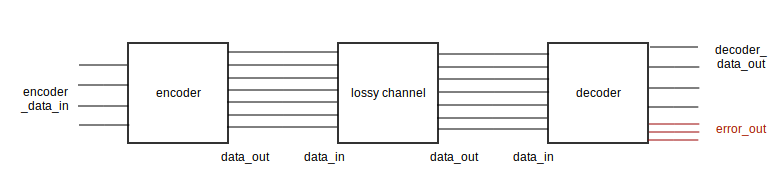
\includegraphics[width=16cm]{flowschema}
				\end{figure}
			\subsection{test bench}
			Deklaracja komponentów do testu:
				\begin{minted}{vhdl}
COMPONENT lossy_channel
GENERIC (N : positive);
PORT(
data_in : IN  std_logic_vector(N-1 downto 0);
clk : IN  std_logic;
data_out : OUT  std_logic_vector(N-1 downto 0)
);
END COMPONENT;

COMPONENT encoder IS
PORT(
data_in : IN  std_logic_vector(3 downto 0);
data_out : OUT  std_logic_vector(6 downto 0)
);
END COMPONENT;

COMPONENT decoder IS
PORT(
data_out: out std_logic_vector(3 downto 0);
data_in: in std_logic_vector(6 downto 0);
error_out: out std_logic_vector(2 downto 0)
);
END COMPONENT;
	
				\end{minted}
				Zestawienie \texttt{encode} i {\texttt{decode} po dwóch stronach kanału.
				\begin{minted}{vhdl}

uut: lossy_channel 
GENERIC MAP ( N => WIDTH )
PORT MAP (
data_in => data_in,
clk => clk,
data_out => data_out
);

eencoder: encoder
PORT MAP(
data_in => encoder_data_in,
data_out => data_in
);

ddecoder: decoder
PORT MAP(
data_in => data_out,
error_out => error_out,
data_out => decoder_data_out
);	
				\end{minted}
				
			\section{Sprawdzenie poprawności działania}
			\subsection{Kanał stratny}
			\begin{figure}[H]
				\centering
				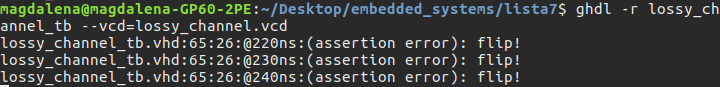
\includegraphics[width=16cm]{terminal}
				\caption{Kanał stratny bez kodowania Hamminga}
			\end{figure}
			
			Przesłanie przez kanał stratny kolejno danych liczbowych od 0 do 15\footnote{Stosujemy szerokość kanału taką jakiej wymaga kodowanie Hamminga w celu umożliwienia porównania. Dlatego dane liczbowe 0-15, które wymagają maksymalnie 4 bitów dopełniane są przez '0' od lewej do szerokości 7 bitów.} zakłamane zostaje 3 krotnie. Błedy zgłaszane są przez asercję w momentach 220ns, 230ns i 240ns.
			
			\begin{figure}[H]
				\centering
				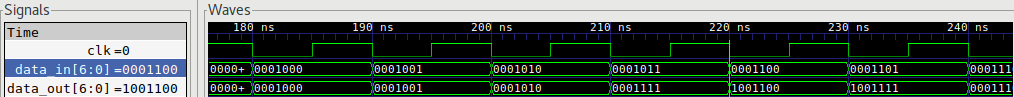
\includegraphics[width=\textwidth]{gtk}
				\caption{Wykres poziomów sygnałów kanału stratnego}
			\end{figure}
			
			Na wykresie widać, że w momencie:
			\begin{itemize}
				\item 220ns zgłoszona została zmiana bitu 3,
				\item 230ns zgłoszona została zmiana bitu 7,
				\item 240ns zgłoszone zostały zmiany bitów 2 i 7.
			\end{itemize}
			
			W dwóch przypadkach zmiany dotyczą tylko jednego bitu. Możemy się zabezpieczyć przed utratą danych stosując kodowanie Hamminga.
			
			\subsection{Kanał stratny z kodowaniem Hamminga}
			
			Oczekujemy, że zakłamania jednego bitu danych w przesyle zostaną naprawione dzięku użyciu kodowania Hamminga.
			
			\begin{figure}[H]
				\centering
				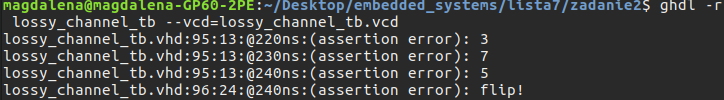
\includegraphics[width=16cm]{ham_terminal}
				\caption{Kanał stratny zabezpieczony przez kodowanie Hamminga}
			\end{figure}
			
			Ponownie zostały przesłane dane liczbowe od 0 do 15, tym razem uzupełnione przez bity parzystości. Wykorzystany generator liczb pseudolosowych LFSR pozwala przy każdym uruchomieniu uzyskać takie samo zachowanie kanału stratnego.
			
			W tym wypadku zakłamanie znów wystąpiło 3 krotnie, jednak błąd w danych wystąpił jedynie raz dzięki zastosowaniu kodowania Hamminga.
			
			\begin{figure}[H]
				\centering
				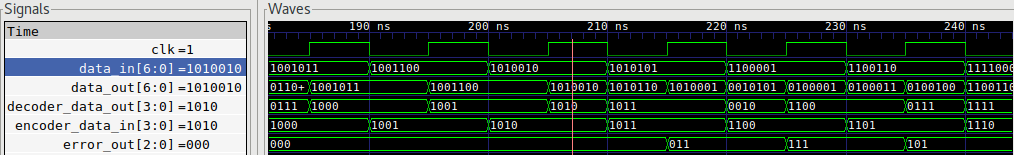
\includegraphics[width=\textwidth]{ham_gtk4}
				\caption{Moment poprawnego przesyłu danych bez zakłamania przez kanał stratny}
			\end{figure}
			
			Gdy kanał stratny nie spowoduje zakłamania, wszystko przebiega poprawnie, \texttt{error\_out} przyjmuje wartość "000".
			
			\begin{figure}[H]
				\centering
				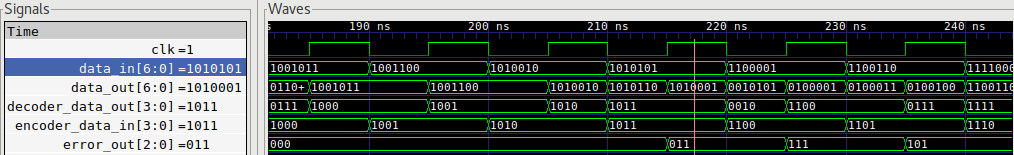
\includegraphics[width=\textwidth]{ham_gtk}
				\caption{Moment przesyłu danych z zakłamaniem 3 bitu przez kanał stratny}
			\end{figure}
			
			\texttt{error\_out} w 220ns wskazuje, że bit 3 został zakłamany w trakcie przesyłu, jednak dane zwrócone przez dekoder są takie same jak te, które zostały zakodowane przed ich wysłaniem. Dzięki kodowaniu Hamminga udało się odzyskać zakłamany bit.
			
			\begin{figure}[H]
				\centering
				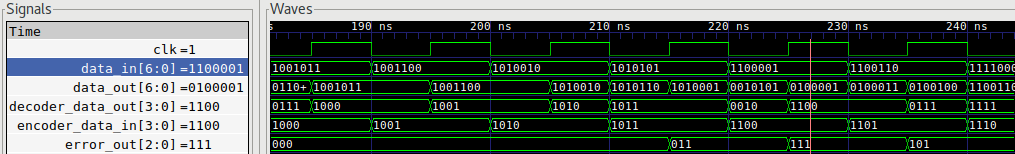
\includegraphics[width=\textwidth]{ham_gtk2}
				\caption{Moment przesyłu danych z zakłamaniem 7 bitu przez kanał stratny}
			\end{figure}
			
			\texttt{error\_out} w 230ns wskazuje, że bit 7 został zakłamany w trakcie przesyłu, jednak dane zwrócone przez dekoder są takie same jak te, które zostały zakodowane przed ich wysłaniem. Dzięki kodowaniu Hamminga udało się odzyskać zakłamany bit.
			
			\begin{figure}[H]
				\centering
				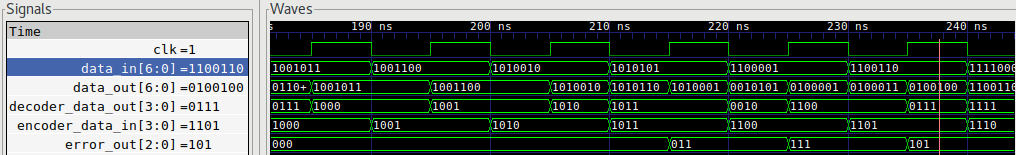
\includegraphics[width=\textwidth]{ham_gtk3}
				\caption{Moment przesyłu danych z zakłamaniem 2 i 7 bitu przez kanał stratny}
			\end{figure}

			\texttt{error\_out} w 240ns wskazuje, że bit 5 został zakłamany w trakcie przesyłu, jednak po analizie wartości \texttt{data\_in} oraz \texttt{data\_out} widać, że zakłamaniu uległy bity 2 i 7. Ponieważ zmiana dotyczy dwóch bitów, kodowanie Hamminga nie było w stanie naprawić błędu, a dane zwrócone przez dekoder są inne niż zakodowane przed wysłaniem. 

\end{document}